\chapter{Spektrales Lernen auf Graphen}
\label{spektrales_lernen}

Das spektrale Lernen auf Graphen \bzw{} die Formulierung eines spektralen Faltungsoperator auf Graphen basiert auf der spektralen Graphentheorie, \dhe{} der Betrachtung des Spektrums eines Graphen definiert über dessen Eigenwerte.
Merkmale auf den Knoten eines Graphen können über das Spektrum analog zur Fourier-Transformation in dessen Frequenzraum zerlegt und wieder retransformiert werden.
Diese Transformation erlaubt damit die fundamentale Formulierung eines Faltungsoperators in der spektralen Domäne des Graphen.
Da der so definierte spektrale Faltungsoperator insbesondere rotationsinvariant ist, wird dieser im Verlauf des Kapitels für den Kontext von Graphen im euklidischen Raum modifiziert.

Durch die spektrale Formulierung kann weiterhin ein effizientes Pooling auf Graphen formuliert werden, welches uns erlaubt, Netzarchitekturen auf Graphen völlig analog zu klassischen \glspl{CNN} auf zweidimensionalen Bildern zu generieren.

\section{Spektrale Graphentheorie}
\label{spektrale_graphentheorie}

Es gibt 2 große Quellen hier:
\begin{itemize}
  \item Spectral Graph Theory by Chung
  \item Discrete Laplace-Beltrami Operator
\end{itemize}
+ 5 zum Lernen:
\begin{itemize}
  \item Semi Supervised Classification
  \item Fast Localized Spectral Filterung
  \item Wavelets on Graphs via Spectral Graph Theory
  \item The Emerging Field of Signal Processing on Graphs
  \item How powerful are Graph Convolutions? (Review)
\end{itemize}

\subsection{Eigenwerte und Eigenvektoren reell symmetrischer Matrizen}
\label{eigenwerte_symmetrischer_matrizen}

\todo{intro}

$\ma{M} \in \gls{R}^{N \times N}$.
$\gls{eiv} \in \gls{R}^{N}$, $\gls{eiv} \neq \mathbf{0}$.
$\gls{lambda} \in \gls{R}$.
\emph{Eigenwertproblem} $\ma{M}\gls{eiv} = \gls{lambda}\gls{eiv}$.
Zu einem \emph{Eigenwert} $\gls{lambda}$ gibt es unendlich viele (skalierte) \emph{Eigenvektoren} \gls{eiv}.
Wir definieren den Eigenvektor \gls{eiv} eines Eigenwertes \gls{lambda} daher eindeutig über die Bedingung $\left\|\gls{eiv}\right\|_2 = 1$.
Sei \ma{M} weiterhin symmetrisch, \dhe{} $\ma{M} = \ma{M}^{\top}$.
Dann gilt für zwei unterschiedliche Eigenvektoren $\gls{eiv}_1$ und $\gls{eiv}_2$, dass $\gls{eiv}_1 \gls{ortho} \gls{eiv}_2$.
Weiterhin hat \ma{M} genau $N$ reelle Eigenwerte mit ${\left\{\gls{lambda}_i\right\}}_{i=1}^N$.

Wir definieren zu \ma{M} die orthogonale \emph{Eigenvektormatrix} $\gls{Eiv} \coloneqq \left[\gls{eiv}_1, \ldots, \gls{eiv}_n\right] \in \gls{R}^{N \times N}$, wobei $\gls{Eiv}\gls{Eiv}^{\top}=\gls{I}$, und dessen korrespondierende Eigenwertdiagonalmatrix $\gls{Lambda} \coloneqq \gls{diag}\left({\left[\gls{lambda}_1, \ldots, \gls{lambda}_N\right]}^{\top}\right)$, \dhe{} $\gls{Lambda}_{ii} = \gls{lambda}_i$.
Dann gilt $\ma{M}\gls{Eiv} = \gls{Eiv}\gls{Lambda}$ und insbesondere ist \ma{M} diagonalisierbar über
\begin{equation*}
  \ma{M} = \ma{M}\gls{Eiv}\gls{Eiv}^{\top} = \gls{Eiv}\gls{Lambda}\gls{Eiv}^{\top}.
\end{equation*}

Weiterhin gilt für die $k$te Potenz von $\ma{M}$, $k \in \gls{N}$,
\begin{equation}
  \ma{M}^k = {\left(\gls{Eiv}\gls{Lambda}\gls{Eiv}^{\top}\right)}^k = \gls{Eiv}\gls{Lambda}^k\gls{Eiv}^{\top}.
  \label{eq:matrix_potenz}
\end{equation}

Dieser Zusammenhang lässt sich verdeutlichen, wenn man die Potenz ausschreibt:
\begin{equation*}
  {\left(\gls{Eiv}\gls{Lambda}\gls{Eiv}^{\top}\right)}^k = \gls{Eiv}\gls{Lambda}\gls{Eiv}^{\top}\gls{Eiv}\gls{Lambda}\gls{Eiv}^{\top}\prod^{k-2}_{i=1} \gls{Eiv}\gls{Lambda}\gls{Eiv}^{\top} = \gls{Eiv}\gls{Lambda}^2\gls{Eiv}^{\top} \prod^{k-2}_{i=1} \gls{Eiv}\gls{Lambda}\gls{Eiv}^{\top} = \gls{Eiv}\gls{Lambda}^k \gls{Eiv}^{\top}.
\end{equation*}

Falls \ma{M} weiterhin \emph{schwach diagonaldominant} ist, \dhe{}
\begin{equation}
  \sum_{\substack{j=1\\j \neq i}}^N \left|\ma{M}_{ij}\right| \leq \left|\ma{M}\right|_{ii},
  \label{eq:schwach_diagonaldominant}
\end{equation}
und weiterhin $\ma{M}_{ii} \geq 0$ für alle $i \in \left\{1, \ldots, N\right\}$, dann ist \ma{M} \emph{positiv semidefinit}, \dhe{} $\ve{x}^{\top}\ma{M}\ve{x} \geq 0$ für alle $\ve{x} \in \gls{R}^{N}$.
Eigenwerte symmetrischer positiv semidefiniter Matrizen $\lambda_i \in \gls{R+}$ sind positiv reell und es lässt sich folglich auf diesen eine Ordnung definieren mit $0 \leq \gls{lambda}_1 \leq \cdots \leq \gls{lambda}_N \coloneqq \gls{lambdamax}$.

\todo{quelle}

\subsection{Laplace-Matrix}
\label{laplace_matrix}

Our eigenvalues relate well to other graph invariants for general graphs in a way that other definitions (such as the eigenvalues of adjacency matrices) often fail to do.
The advantages of this definition are perhaps due to the fact that it is consistent with the eigenvalues in spectral geometry and in stochastic processes.
Many results which were only known for regular graphs can be generalized to all graphs~\cite{Chung}.

\todo{intro}

Für einen schleifenlosen, ungerichteteten, gewichtet oder ungewichteten Graphen \gls{G} und dessen Adjazenzmatrix \gls{A} mit Gradmatrix \gls{D} ist die \emph{kombinatorische Laplace-Matrix} \gls{L} definiert als $\gls{L} \coloneqq \gls{D} - \gls{A}$~\cite{Chung}.
Die \emph{normalisierte Laplace-Matrix} \gls{Lnorm} ist definiert als $\gls{Lnorm} \coloneqq \gls{D}^{-\frac{1}{2}} \gls{L} \gls{D}^{-\frac{1}{2}}$ mit der Konvention, dass $\gls{D}^{-\frac{1}{2}}_{ii} = 0$ für isolierte Knoten $\gls{v}_i \in \gls{V}$ in \gls{G}, \dhe{} $\gls{D}_{ii} = 0$~\cite{Chung}.
Daraus ergibt sich die elementweise Definition
\begin{equation*}
  \gls{Lnorm}_{ij} \coloneqq \begin{cases}
  1, & \text{wenn }i = j,\\
    -\frac{\gls{w}\left(\gls{v}_i, \gls{v}_j\right)}{\sqrt{\gls{d}\left(\gls{v}_i\right)\gls{d}\left(\gls{v}_j\right)}}, & \text{wenn }\gls{v}_i \gls{adj} \gls{v}_j,\\
  0, & \text{sonst.}
\end{cases}
\end{equation*}
Für verbundene Graphen kann \gls{Lnorm} vereinfacht werden zu $\gls{Lnorm} \coloneqq \gls{I} - \gls{D}^{-\frac{1}{2}} \gls{A} \gls{D}^{-\frac{1}{2}}$~\cite{Chung}.
Jeder Eintrag auf der Diagonalen der normalisierten Laplace-Matrix ist folglich Eins.
\gls{Lnorm} ist damit normalisiert auf den (gewichteten) Grad zweier adjazenter Knoten $\gls{v}_i$ und $\gls{v}_j$.
Es ist anzumerken, dass \gls{L} und insbesondere \gls{Lnorm} symmetrisch sind, wohingegen eine Normalisierung der Form $\gls{D}^{-1}\gls{L}$ dies in der Regel nicht wäre~\cite{Reuter}.

\gls{L} und \gls{Lnorm} sind keine ähnlichen Matrizen.
Insbesondere sind ihre Eigenvektoren unterschiedlich.
Die Nutzung von \gls{L} oder \gls{Lnorm} ist damit abhängig von dem Problem, welches man betrachtet~\cite{Hammond}.
Wir schreiben \gls{Lboth} wenn die Wahl der Laplace-Matrix, ob \gls{L} oder \gls{Lnorm}, für die weitere Berechnung zwar fest, aber irrelevant ist.

\paragraph{Interpretation}
\label{laplace_interpretation}

\todo{kurz laplace beltrami}

Sei $\ve{f} \in \gls{R}^N$ eine Funktion \bzw{} ein Signal auf den Knoten eines Graphen \gls{G}.
Dann kann für die kombinatorische Laplace-Matrix \gls{L} verifiziert werden, dass \gls{L} die Gleichung
\begin{equation*}
  {\left(\gls{L}\ve{f}\right)}_i = \sum_{i \gls{adj} j} \gls{w}\left(\gls{v}_i, \gls{v}_j\right) \left(\ve{f}_i - \ve{f}_j\right)
\end{equation*}
erfüllt~\cite{Hammond}.
Sei $\gls{G}$ nun ein Graph, der aus einem (unendlichen) zweidimensionalen regulärem Gitter entstanden ist, \dhe{} jeder Knoten $\gls{v}_i$ besitzt genau $4$ Nachbarn mit gleichen Kantengewichten $\frac{1}{\delta^2}$, wobei $\delta \in \gls{R}$ beliebige Konstante.
Zur einfacheren Veranschaulichung benutzen wir dabei für die Signalstärke $\ve{f}_i$ eines Knoten $v_i$ an Position $\left(x, y\right)$ die Indexnotation $\ve{f}_{x,y}$.
Dann beschreibt
\begin{equation*}
  {\left(\gls{L}\ve{f}\right)}_{x,y} = \frac{4\ve{f}_{x,y} - \ve{f}_{x+1,y} - \ve{f}_{x-1,y} - \ve{f}_{x,y+1} - \ve{f}_{x,y-1}}{h^2}
\end{equation*}
die \emph{5-Punkte-Stern} Approximation $-\nabla^2 f$ (bei umgekehrtem Vorzeichen) definiert auf den Punkten $\left\{\left(x,y\right), \left(x+\delta,y\right), \left(x-\delta,y\right), \left(x,\delta+h\right),\left(x,y-\delta\right)\right\}$~\cite{Hammond}.\todo{grafik}
Ähnlich zu einem regulären Gitter lässt sich ein Graph \gls{G} auch über beliebig viele Abtastpunkte einer differenzierbaren Mannigfaltigkeit konstruieren.
Es zeigt sich, dass mit steigender Abtastdichte und geeigneter Wahl der Kantengewichte die normalisierte Laplace-Matrix \gls{Lnorm} zu dem kontinuierlichem Laplace-Beltrami Operator konvergiert~\cite{Hammond}.
Damit kann $\gls{Lnorm}$ als die diskrete Analogie des $\nabla^2$ Operators auf Graphen verstanden werden.
Der Laplace-Beltrami Operator misst dabei, in wie weit sich eine Funktion $f$ an einem Punkt $x$ von dem Durchschnitt aller Funktionspunkte um einen kleinen Bereich um $x$ unterscheidet.
Die Laplace-Matrix operiert dabei völlig analog, in dem sie misst, wie sehr sich eine (diskrete) Funktion um einen Knoten im Vergleich zu seinen Nachbarknoten unterscheidet.

Eigenwerte und Eigenvektoren von \gls{Lboth} helfen uns dabei, die lineare Transformation einer Funktion \ve{f} (mehrfach) angewendet auf \gls{Lboth} besser zu verstehen.
Wir können dafür \ve{f} als Linearkombination der Eigenbasis $\sum_i c_i \gls{eiv}_i$ schreiben und erhalten
\begin{equation*}
  \gls{Lboth}^k \ve{f} = \sum_i c_i \gls{Lboth}^k \gls{eiv}_i = \sum_i c_i \gls{lambda}_i^k \gls{eiv}_i.
\end{equation*}
Somit können Eigenschaften von \gls{Lboth} und damit des Graphen selber durch dessen Eigenwerte und Eigenvektoren beschrieben werden.

\paragraph{Eigenschaften}
\label{laplace_eigenschaften}

$\gls{Lboth} \in \gls{R}^{N \times N}$ ist eine reell symmetrisch, positiv semidefinite Matrix~\cite{Chung}.
Folglich besitzt \gls{Lboth} nach Kapitel~\ref{eigenwerte_symmetrischer_matrizen} genau $N$ positiv reelle Eigenwerte ${\left\{\gls{lambda}_i\right\}}_{i=1}^N$ mit Ordnung $0 \leq \gls{lambda}_1 \leq \cdots \leq \gls{lambda}_N$ und $N$ korrespondierende orthogonale Eigenvektoren ${\left\{\gls{eiv}_i\right\}}_{i=1}^N$.

Die kombinatorische Laplace-Matrix $\gls{L}$ ist nach~\eqref{eq:schwach_diagonaldominant} weiterhin schwach diagonaldominant.
Insbesondere summiert sich jede Reihen- und Spaltensumme von \gls{L} zu Null auf, \dhe{} $\sum_{j=1}^N \gls{L}_{ij} = \sum_{j=1}^N \gls{L}_{ji} = 0$.
Daraus folgt unmittelbar, dass $\gls{lambda}_1 = 0$, da $\gls{eiv}_1 = \frac{1}{\sqrt{N}}{\left[1, \ldots, 1\right]}^{\top} \in \gls{R}^N$ Eigenvektor von \gls{L} mit $\gls{L}\gls{eiv}_1 = \ve{0}$.
\gls{Lnorm} hingegen ist nicht zwingend schwach diagonaldominant.
Es lässt sich jedoch zeigen, dass auch für \gls{Lnorm} gilt, dass $\gls{lambda}_1 = 0$~\cite{Chung}.

Eine der interessantesten Eigenschaften eines Graphs ist dessen Konnektivität.
Die Laplace-Matrix \gls{Lboth} \bzw{} dessen Eigenwerte stellen ein geeignetes Mittel zur Untersuchung dieser Eigenschaft dar.
So gilt \zB{} für einen verbundenen Graphen \gls{G}, dass $\gls{lambda}_2 > 0$.
Falls $\gls{lambda}_i = 0$ und $\gls{lambda}_{i+1} \neq 0$, dann besitzt $\gls{G}$ genau $i$ verbundene Komponenten~\cite{Chung}.
Damit ist die Anzahl der Null-Eigenwerte äquivalent zu der Anzahl an Komponenten, die ein Graph besitzt.
Für \gls{Lnorm} lässt sich weiterhin zeigen, dass $\gls{lambdamax} \leq 2$ eine obere Schranke ihrer Eigenwerte ist~\cite{Chung}.

Aus der Laplace-Matrix können ebenso Rückschlüsse über die kürzeste Pfaddistanz zweier Knoten gewonnen werden.
So gilt für $\gls{Lboth}^{k}$ mit $k \in \gls{N}$, dass $\gls{Lboth}^k_{ij} = 0$ genau dann, wenn $\gls{s}\left(v_i, v_j\right) > k$~\cite{Hammond}.
Damit beschreibt $\gls{Lboth}^k_i$ bildlich gesprochen die Menge an Knoten, die maximal $k$ Kanten von $i$ entfernt liegen.

\section{Spektraler Faltungsoperator}
\label{spektraler_faltungsoperator}

\subsection{Graph-Fourier-Transformation}
\label{graph_fourier_transformation}

\subsection{Polynomielle Approximation}
\label{polynomielle_approximation}

\paragraph{Tschebyschow-Polynome}
\label{tschebyschow_polynome}

\section{Graph Convolutional Networks}
\label{graph_convolutional_networks}

\citeauthor{gcn} motivieren einen weiteren Ansatz zur Faltung auf Graphen, genannt \emph{\gls{GCN}}, der auf der Methodik des spekralen Faltungsoperators aus Kapitel~\ref{spektraler_faltungsoperator} aufbaut und dabei wie eine \enquote{differenzierbare und parametrisierte Generalisierung des eindimensionalen Weisfeiler-Lehman Algorithmus auf Graphen} fungiert~\cite{gcn}.

\paragraph{Faltungsoperator}
\label{gcn_faltungsoperator}

Sei $\ve{f}_{\mathrm{in}} \star \ve{\hat g} \approx \sum_{k=0}^K c_k \gls{T}_k\left(\gls{Lbothtilde}\right) \ve{f}_{\mathrm{in}}$ der in~\eqref{eq:tschebyschow_faltung_L} definierte spektrale Faltungsoperator mit $K=1$.
Dann ist $\ve{f}_{\mathrm{in}} \star \ve{\hat g}$ eine lineare Funktion \bzgl{} \gls{Lboth} und damit eine lineare Funktion auf dem Spektrum des Graphen~\cite{gcn}.
Mit $K=1$ betrachtet der spektrale Faltungsoperator nur noch die lokale Nachbarschaft eines jeden Knotens (\vgl{}~\ref{polynomielle_approximation}).
Es ist anzumerken, dass dies in der Regel keinen Nachteil darstellt.
So hat es sich bei gegenwärtigen \enquote{State-of-the-Art}-\glspl{CNN} auf Bildern ebenfalls eingebürgert, nur noch über minimale $3\times3$ Filtergrößen zu falten und stattdessen Merkmale weit entfernterer Knoten über die mehrfache Aneinanderreihung der Faltungsschichten mittels tieferer Netze zu gewinnen~(\vgl{}~\cite{gcn, vgg, He}).
Unter dieser Restriktion vereinfacht sich $\ve{f}_{\mathrm{in}} \star \ve{\hat g}$ zu
\begin{equation}
  \ve{f}_{\mathrm{in}} \star \ve{\hat g} \approx c_0\, \ve{f}_{\mathrm{in}} + c_1 \left(\frac{2}{\gls{lambdamax}}\gls{Lboth} - \gls{I}\right)\ve{f}_{\mathrm{in}}
  \label{eq:gcn_faltung_both}
\end{equation}
mit zwei freien Parametern $c_0$ und $c_1$~\cite{gcn}.
Für $\gls{Lnorm}$ auf einem zusammenhängenden Graphen \gls{G} gilt dann nach~\eqref{eq:gcn_faltung_both} weiter
\begin{equation}
  \ve{f}_{\mathrm{in}} \star \ve{\hat g} \approx c_0 \, \ve{f}_{\mathrm{in}} + c_1 \left(\gls{Lnorm} - \gls{I}\right)\ve{f}_{\mathrm{in}} = c_0 \, \ve{f}_{\mathrm{in}} - c_1 \gls{D}^{-\frac{1}{2}} \gls{A} \gls{D}^{-\frac{1}{2}} \ve{f}_{\mathrm{in}},
  \label{eq:gcn_faltung_norm}
\end{equation}
wobei $\gls{lambdamax} \coloneqq 2$ auf dessen obere Schranke gesetzt wird~\cite{gcn}.
Um die Gefahr des Overfittings und die Anzahl an Berechnungen pro Schicht weiter zu beschränken, reduziert sich~\eqref{eq:gcn_faltung_norm} mit einem einzigen Parameter $c \coloneqq c_0$ mit $c = -c_1$ zu~\cite{gcn}
\begin{equation*}
  \ve{f}_{\mathrm{in}} \star \ve{\hat g} \approx c \left(\gls{I} + \gls{D}^{-\frac{1}{2}} \gls{A} \gls{D}^{-\frac{1}{2}} \right) \ve{f}_{\mathrm{in}}.
\end{equation*}
Die skalierten Eigenwerte von \gls{Lambdatilde} liegen auf Grund der Addition mit \gls{I} nun im Intervall $\left[0, 2\right]$ (\vgl{}~\cite{gcn}).
Demnach können wiederholte Anwendungen des Faltungsoperators zu \enquote{numerischen Instabilitäten und folglich zu explodierenden oder verschwindenen Gradienten} führen~\cite{gcn}.
\citeauthor{gcn} führen zur Behebung dieses Problems die folgende Renormalisierung durch: $\gls{I} + \gls{D}^{-1/2} \gls{A} \gls{D}^{-1/2} \rightarrow \gls{Dtilde}^{-1/2} \gls{Atilde} \gls{Dtilde}^{-1/2}$ mit $\gls{Atilde} \coloneqq \gls{A} + \gls{I}$ und $\gls{Dtilde}_{ii} \coloneqq \sum_{j=1}^N \gls{Atilde}_{ij}$.
Der entgültige Faltungsoperator des \glspl{GCN} ergibt sich dann als
\begin{equation}
  \ve{f}_{\mathrm{in}} \star \ve{\hat g} \approx c\, \gls{Dtilde}^{-\frac{1}{2}} \gls{Atilde} \gls{Dtilde}^{-\frac{1}{2}} \ve{f}_{\mathrm{in}}
  \label{eq:gcn_renorm}
\end{equation}
auf einem einzigen freien Parameter $c \in \gls{R}$.

\paragraph{Implementierung}
\label{gcn_tensor}

Die Faltung des \glspl{GCN} auf Merkmalsmatrizen lässt sich analog zur Tensorimplementierung des spektralen Faltungsoperators in Kapitel~\ref{polynomielle_approximation} beschreiben, mit dem Unterschied, dass wir aufgrund der Festlegung von $K=1$ keinen Filtertensor, sondern lediglich eine Filtermatrix $\gls{W} \in \gls{R}^{M_{\mathrm{in}} \times M_{\mathrm{out}}}$ nutzen.
Die Faltung einer Eingabemerkmalsmatrix $\gls{F}_{\mathrm{in}} \in \gls{R}^{N \times M_{\mathrm{in}}}$ auf eine Ausgabemerkmalsmatrix $\gls{F}_{\mathrm{out}} \in \gls{R}^{N \times M_{\mathrm{out}}}$ ergibt sich dann als
\begin{equation}
  \ma{F}_{\mathrm{out}} \coloneqq \gls{Dtilde}^{-\frac{1}{2}} \gls{Atilde} \gls{Dtilde}^{-\frac{1}{2}}\, \ma{F}_{\mathrm{in}} \gls{W}
  \label{eq:gcn_tensor}
\end{equation}
mit Faltungsaufwand $\gls{O}\left(M_{\mathrm{in}}M_{\mathrm{out}}\left|\gls{E}\right|\right)$, weil $\gls{Atilde}\ma{F}_{\mathrm{in}}$ effizient mit der Multiplikation einer dünnbesetzten mit einer dichtbesetzten Matrix implementiert werden kann~\cite{gcn}.

\paragraph{Beziehung zum Weisfeiler-Lehman Algorithmus}
\label{weisfeiler_lehman_beziehung}

\begin{algorithm}[t]
\centering
\begin{algorithmic}
  \REQUIRE{} Initiale Knotenfärbung $\ve{h}^{\left(0\right)} \in \gls{R}^N$
  \ENSURE{} Finale Knotenfärbung $\ve{h}^{\left(T\right)} \in \gls{R}^N$ nach $T$ Durchläufen
  \STATE{} $t \leftarrow 0$
  \REPEAT{}
    \FOR{$\gls{v}_i \in \gls{V}$}
      \STATE{} $\ve{h}^{\left(t+1\right)}_i \leftarrow \mathrm{hash}\left(\sum_{\gls{v}_j \in \gls{Neighbor}\left(\gls{v}_i\right)} \ve{h}^{\left(t\right)}_j\right)$
    \ENDFOR{}
    \STATE{} $t \leftarrow t + 1$
  \UNTIL{Konvergenz}
\end{algorithmic}
  \caption[Weisfeiler-Lehman Algorithmus]{Eindimensionaler Weisfeiler-Lehman Algorithmus auf einer initialen Knotenfärbung $\ve{h}^{\left(0\right)} \in \gls{R}^N$ eines Graphen \gls{G} mit $\gls{v}_i \in \gls{Neighbor}\left(\gls{v}_i\right)$~\cite{wl}.}
\label{alg:wl}
\end{algorithm}

Der \emph{eindimensionale Weis\-fei\-ler-Lehman Algorithmus} beschreibt eine weit-untersuchte Methode zur Knotenklassifizierung eines Graphen basierend auf einer intialen Färbung \bzw{} Merkmalsverteilung auf den Knoten eines Graphen \gls{G}, die unteranderem zur Bestimmung von Graphisomorphismen genutzt wird~\cite{douglas}.
Basierend auf einer intialen Knotenfärbung $\ve{h}^{\left(0\right)} \in \gls{R}^N$ wird die Farbe eines jeden Knotens $\gls{v}_i \in \gls{V}$ sukzessive mit Hilfe einer Hashfunktion $\mathrm{hash}\left(\cdot\right)$ so angepasst, dass sie die vorangegangene Farbe des Knotens zusammen mit den Farben seiner lokalen Nachbarschaft repräsentiert.
Dieser Prozess wiederholt sich solange, bis eine stabile Knotenfärbung gefunden wurde, \dhe{} die gefundene Färbung des Graphen konvergiert (\vgl{} Algorithmus~\ref{alg:wl}).

Sei die Hashfunktion gegeben als eine differenzierbare, nicht-lineare Aktivierungsfunktion $\gls{act}\left(\cdot\right)$ eines neuronalen Netzes.
Dann ergibt sich die Faltung des \glspl{GCN} als
\begin{equation*}
  \ve{h}^{\left(t+1\right)}_i = \gls{act}\left(\sum_{\gls{v}_j \in \gls{Neighbor}\left(\gls{v}_i\right)} \frac{1}{\sqrt{d_i d_j}} \ve{h}^{\left(l\right)}_j \gls{W} \right),
\end{equation*}
wobei $1/\sqrt{d_i d_j} \in \gls{R}$ eine Normalisierungskonstante für die Kante $\left(\gls{v}_i, \gls{v}_j\right) \in \gls{E}$ ist~\cite{gcn}.
Damit kann die Faltung des \glspl{GCN} als \enquote{differenzierbare und parametrisierte Generalisierung des eindimensionalen Weisfeiler-Lehman Algorithmus auf Graphen} verstanden werden~\cite{gcn}.

\section{Erweiterung auf Graphen im zweidimensionalen euklidschen Raum}
\label{gcn_erweiterung}

Die Ansätze von~\citeauthor{Defferrard} aus Kapitel~\ref{spektraler_faltungsoperator} und~\citeauthor{gcn} aus Kapitel~\ref{graph_convolutional_networks} zeigen konkurrenzfähige Resultate auf einer Reihe von Datensätzen auf Graphen (\vgl{}~\cite{Defferrard, gcn}).
So erreicht das \gls{GCN} \zB{} in der teilweise-überwachten Knotenklassifizierung von Referenz-Graphen, \dhe{} einer Menge von Knoten, die Dokumente über eine Reihe von Bag-of-Words-Merkmalen repräsentieren und (ungerichtet) über dessen Referenzierungen miteinander verbunden sind, beachtliche Ergebnisse und schneidet in diesen sogar knapp besser ab als über die Tschebyschow-Approximation mit $K=2$ und $K=3$~\cite{gcn}.

Die spektrale Faltung auf Graphen entspricht einer Generalisierung der Faltung klassischer \glspl{CNN} auf zweidimensionalen Bildern~\cite{gcn_review}.
Es ist jedoch anzumerken, dass die spektrale Faltung im Gegensatz zur klassischen Faltung auf einem regulären Gitter insbesondere rotationsinvariant ist.
Das ist in der Regel für generelle Graphen keine Schwäche, schließlich kann den Knoten \bzw{} Kanten eines Graphen, kodiert als Adjazenzmatrix, keine Örtlichkeit \bzw{} Richtung (wie links, rechts, oben oder unten) zugeordnet werden.
Die Rotationsinvarianz kann folglich sowohl als Einschränkung oder Vorteil interpretiert werden, abhängig von dem Problem, welches man betrachtet~\cite{Defferrard}.

\begin{figure}[t]
\centering
\subfigure[Reguläres Gitter]{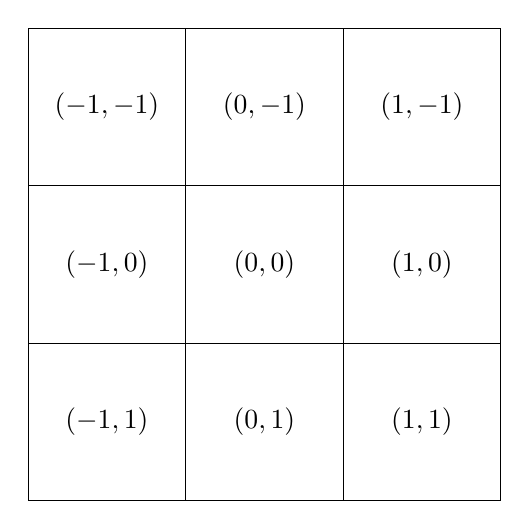
\begin{tikzpicture}
  \draw (-3, -3) rectangle (-1, -1) node[pos=0.5] {$\left(-1, 1\right)$};
  \draw (-1, -3) rectangle (1, -1)  node[pos=0.5] {$\left(0, 1\right)$};
  \draw (1, -3)  rectangle (3, -1)  node[pos=0.5] {$\left(1, 1\right)$};
  \draw (-3, -1) rectangle (-1, 1)  node[pos=0.5] {$\left(-1, 0\right)$};
  \draw (-1, -1) rectangle (1, 1)   node[pos=0.5] {$\left(0, 0\right)$};
  \draw (1, -1)  rectangle (3, 1)   node[pos=0.5] {$\left(1, 0\right)$};
  \draw (-3, 1)  rectangle (-1, 3)  node[pos=0.5] {$\left(-1, -1\right)$};
  \draw (-1, 1)  rectangle (1, 3)   node[pos=0.5] {$\left(0, -1\right)$};
  \draw (1, 1)   rectangle (3, 3)   node[pos=0.5] {$\left(1, -1\right)$};
\end{tikzpicture}
}
\hspace{1cm}
\subfigure[Graphrepräsentation]{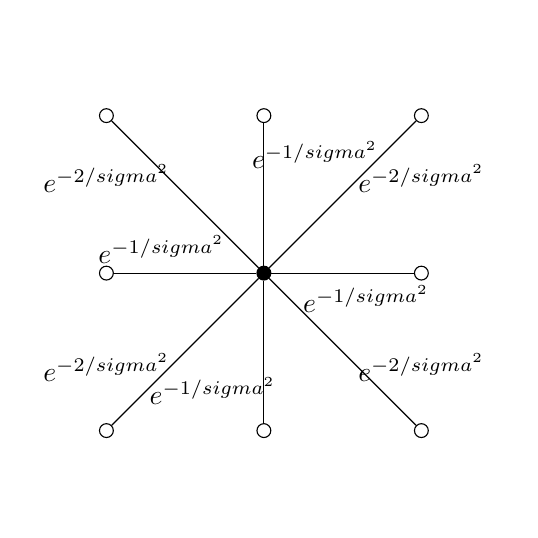
\begin{tikzpicture}
  \tikzstyle{node}=[circle,draw, minimum width=5pt, inner sep=0pt, fill=white]
  \tikzstyle{root}=[fill=black]
  \fill [white] (-3, -3) rectangle (3, 3) node {};  % Zentriere vertikal.

  \node[node] (00) at (-2, 2) {};
  \node[node] (01) at (0, 2) {};
  \node[node] (02) at (2, 2) {};
  \node[node] (10) at (-2, 0) {};
  \node[node, root] (11) at (0,0) {};
  \node[node] (12) at (2, 0) {};
  \node[node] (20) at (-2, -2) {};
  \node[node] (21) at (0, -2) {};
  \node[node] (22) at (2, -2) {};

  \path (10) edge node[shift={(-0.3, 0.3)}]  {$e^{-1/\gls{sigma}^2}$} (11);
  \path (11) edge node[shift={(0.3, -0.33)}]  {$e^{-1/\gls{sigma}^2}$} (12);
  \path (01) edge node[shift={(0.65, 0.5)}]   {$e^{-1/\gls{sigma}^2}$} (11);
  \path (11) edge node[shift={(-0.65, -0.5)}] {$e^{-1/\gls{sigma}^2}$} (21);
  \path (00) edge node[shift={(-1, 0.2)}]    {$e^{-2/\gls{sigma}^2}$} (11);
  \path (02) edge node[shift={(1, 0.2)}]     {$e^{-2/\gls{sigma}^2}$} (11);
  \path (11) edge node[shift={(1, -0.2)}]    {$e^{-2/\gls{sigma}^2}$} (22);
  \path (20) edge node[shift={(-1, -0.2)}]   {$e^{-2/\gls{sigma}^2}$} (11);
\end{tikzpicture}
}
  \caption[Graphrepräsentation eines regulären Gitters]{Illustration (a) eines $3 \times 3$ großen regulären Gitters zentriert um den Punkt $\left(0, 0\right)$ und (b) dessen lokale Nachbarschaft der entsprechenden Graphrepräsentation mit einer Konnektivität von $8$ bei horizontalen \bzw{} vertikalen Kantengewichten $\exp\left(-1/\gls{sigma}^2\right) \in \gls{R}$ und respektive $\exp\left(-2/\gls{sigma}^2\right) \in \gls{R}$ bei den Diagonalen.}
\label{fig:gcn_review}
\end{figure}


Im Kontext dieser Arbeit, dem Lernen auf Graphen im zweidimensionalen euklidschen Raum, bei denen Graphknoten eine eindeutige Position besitzen, ist die Rotationsinvarianz weitestgehend unerwünscht.
Das kann leicht verifiziert werden, indem wir den Filter des \glspl{GCN} auf einer Graphrepräsentation eines Gitters mit Abstand $\left\|1\right\|_2$ visualisieren (vgl. Abbildung~\ref{fig:gcn_review}).
Diese Repräsentation entspricht damit genau dem Problem der zweidimensionalen Faltung auf Bildern mit einer Filtergröße von $3 \times 3$.
Hier zeigt sich jedoch besonders deutlich die Limitierung des Netzes durch die Rotationsinvarianz.
Wohingegen wir bei klassischen \glspl{CNN} $3 \times 3$ unterschiedliche Parameter mit eindeutiger Örtlichkeit auf den benachbarten Bildpixeln trainieren, reduziert sich der Filter des \glspl{GCN} (vereinfacht ohne Normalisierung mit $\gls{Dtilde}^{-1/2}$) effektiv zu einer Filtermatrix der Form
\begin{equation*}
  \begin{bmatrix}
    ce^{-2/\gls{sigma}^2} & ce^{-1/\gls{sigma}^2} & ce^{-2/\gls{sigma}^2}\\
    ce^{-1/\gls{sigma}^2} & c & ce^{-1/\gls{sigma}^2}\\
    ce^{-2/\gls{sigma}^2} & ce^{-1/\gls{sigma}^2} & ce^{-2/\gls{sigma}^2}
  \end{bmatrix} = c \begin{bmatrix}
    e^{-2/\gls{sigma}^2} & e^{-1/\gls{sigma}^2} & e^{-2/\gls{sigma}^2}\\
    e^{-1/\gls{sigma}^2} & 1 & e^{-1/\gls{sigma}^2}\\
    e^{-2/\gls{sigma}^2} & e^{-1/\gls{sigma}^2} & e^{-2/\gls{sigma}^2}
  \end{bmatrix}
\end{equation*}
mit einem einzigen trainierbaren Parameter $c \in \gls{R}$ bei horizontalen \bzw{} vertikalen Kantengewichten $\exp\left(-1/\gls{sigma}^2\right) \in \gls{R}$ und respektive $\exp\left(-2/\gls{sigma}^2\right) \in \gls{R}$ bei den Diagonalen.
Damit reduziert sich das Training einer Faltungsschicht eines solchen \glspl{GCN} letztendlich auf eine Skalarmultiplikation.
Es erscheint fast unmöglich mit diesem Ansatz komplexe Probleme wie \zB{} Bildsegementierung oder ähnlichem zu lösen~(\vgl{}~\cite{gcn_review}).
Ein Vergleich zwischen der spektralen Faltung auf regulären Gittergraphen und der klassischen zweidimensionalen Faltung auf Bildern wird der spektralen Faltung aber nicht gerecht, schließlich wurden die klassischen \glspl{CNN} speziell für die Anwendung auf Gittern entwickelt.
So ist es zu erwarten, dass durch die Formulierung einer Faltung für generelle Graphen gewisse Einschränkungen in Kauf genommen werden müssen.
Im Folgenden lässt sich der Faltungsoperator der \glspl{GCN} aber insofern modifizieren, dass sich dieser für beliebige Graphen in einem zweidimensionalen euklischen Raum äquivalent zu der klassischen Formulierung auf regulären Gittern verhält.

\subsection{Partitionierung}
\label{partitionierung}

\section{Partitionierung}

\section{Partitionierung}

\input{figures/partitionierung}

\subsection{Grundlagen}

\begin{itemize}
  \item ungerichtete Distanzadjazenzmatrix $\gls{Adist} \in \gls{R+}^{N \times N} = {\left(a\right)}_{ij}$
  \item (lokal) normalisierte ungerichtete Distanzadjazenzmatrix $\gls{Adistnorm} \in \gls{R+}^{N \times N} = {\left(\tilde a\right)}_{ij}$
  \item gerichtete Winkeladjazenzmatrix $\gls{Arad} \in \gls{R+}^{N \times N} = {\left(\alpha\right)}_{ij}$
  \item Input-Featurematrix $\gls{F} \in \gls{R}^{N \times X} = {\left(f\right)}_{ij}$
  \item Output-Featurematrix $\gls{Fout} \in \gls{R}^{N \times Y} = {\left(f^{\prime}\right)}_{ij}$
  \item Anzahl Partitionen $P \in \gls{N}$
  \item Gewichtstensor $\ma{W} \in \gls{R}^{\left(P + 1\right) \times X \times Y} = {\left(w\right)}_{ijw}$
\end{itemize}

\subsection{Faltung}

\begin{equation}
  f^{\prime}_{iy} = \sum_{x = 1}^X \tilde a_{ii} \cdot f_{ix} \cdot w_{\left(P +1\right)xy} \sum_{n = 1, n \neq i}^N \tilde a_{in} \cdot f_{nx} \cdot b^K_P\left(\alpha_{in}, x, y\right)
\end{equation}
wobei $b_P^K$ eine B-Spline-Kurve.

Es ist anzumerken, dass im Summanden der betrachtete Knoten übersprungen wird, da für diesen ein Wert in der Winkelmatrix keinen Sinn ergibt.
Er wird daher in der Faltung jeweils einzeln mit einem Gewicht multipliziert und dazuaddiert.

\subsection{B-Spline-Kurven}

$b_P^K \colon \left]0, 2\pi\right] \times \left\{1, \ldots, X \right\} \times \left\{1, \ldots, Y\right\} \to \gls{R}$ ist eine B-Spline-Kurve der Ordnung $K \in \gls{N}$ auf den Kantenwinkeln des Graphen.
Bemerke, dass wir $0$ für Winkel aussschließen und stattdessen den Winkel $2\pi$ benutzen, so dass wir nicht mit der Bedeutung von $0$ bei Adjazenzmatrizen in die Quere kommen.
\begin{equation}
  b_P^K\left(\alpha, x, y \right) = \sum_{p=1}^P w_{pxy} \cdot e_p^K\left(\alpha\right)
\end{equation}
wobei die Basisfunktion $e_p^K$ rekursiv über $K$ definiert ist mit Initialisierung
\begin{equation}
  e_p^1\left(\alpha\right) = \begin{cases}
    1, & \text{wenn }\alpha \in \left] t\left(p-1\right), t\left(p\right)\right]\text{,}\\
    0, & \text{sonst}
  \end{cases}
\end{equation}
und Rekursionsschritt
\begin{equation}
  e_p^k\left(\alpha\right) = \frac{\alpha - t\left(p - 1\right)}{t\left(p+k-2\right) - t\left(p - 1\right)} e_p^{k-1}\left(\alpha\right) + \frac{t\left(i\left(p + k - 1\right)\right) - \alpha}{t\left(p+k - 1\right) - t\left(p\right)} e_{i\left(p+1\right)}^{k-1}\left(\alpha\right)
\end{equation}
wobei $t \colon \gls{N} \to \gls{R}$ mit $t\left(p\right) = 2\pi\frac{p}{P}$ und $i\left(p\right) = \gls{modulo}\left(p-1, P\right) + 1$.
Es ist anzumerken, dass wir $t$ und $i$ dabei für den Rekursionsschritt über die Grenze $P$ hinaus definieren.
Das hilft uns, die B-Spline-Kurve \emph{kreisförmig} abzuschließen.

Je größer $K$ gesetzt wird, umso mehr Anteile anderer benachbarter Stützpunkte fließen in die Berechnung mit ein.
Die Größe von $K$ wird deshalb auch oft \emph{lokale Kontrollierbarkeit} genannt.

\subsubsection{Beispiel mit $P=4$}

\input{figures/bspline-basis}

\subsubsection{Effiziente Berechnung für $K=2$}

Wir können für $K=2$ die Basis-Berechnung durch
\begin{equation}
  e_p^2\left(\alpha\right) = \begin{cases}
    \min\left(\frac{P}{2\pi} \alpha - p + 1, 0\right), & \text{wenn }\alpha \leq t\left(p\right)\text{,}\\
    \min\left(-\frac{P}{2\pi} \alpha + p + 1, 0\right), & \text{sonst}
  \end{cases}
\end{equation}
vereinfachen.

\begin{proof}
  Aufsteigende Gerade der Dreiecksfunktion für $p$, $1 \leq p \leq P$, ist definiert durch
  \begin{equation}
    \frac{\alpha - t\left(p-1\right)}{t\left(p\right) - t\left(p-1\right)} = \frac{P\left(\alpha - t\left(p-1\right)\right)}{2\pi} = \frac{P\alpha - 2\pi\left(p-1\right)}{2\pi} = \frac{P}{2\pi}\alpha - p + 1.
  \end{equation}
  $\min \left(\frac{P}{2\pi} \alpha - p + 1, 0\right)$ beschreibt damit die linke Seite des Dreiecks.
  Analog für absteigende Gerade.
\end{proof}

Die Fallunterscheidung ist unnötig, wir können uns einfach immer für das Minimum der beiden entscheiden.
Die Grafik zeigt dies ziemlich eindeutig.
Das ergibt letztendlich
\begin{equation}
  e_p^2\left(\alpha\right) = \min \left( \min\left(\frac{P}{2\pi} \alpha - p + 1, 0\right), \min\left(-\frac{P}{2\pi} \alpha + p + 1, 0\right) \right)\text{.}
\end{equation}

\input{figures/bspline-basis-k-2}

Wir haben bisher noch nicht den \emph{Kreis} geschlossen mit unserer Formel.

Das können wir aber leicht tun, indem wir unsere absteigenden Geraden um $2\pi$ nach links verschieben und daraus wiederum das Minimum von $0$ ziehen.
Dann sind diese Geraden außer für $p = P$ im Gültigkeitsbereich der Funktion allesamt $0$.
Wir können demnach aus unserer bisherigen Formel und der verschobenen Gerade das Maximum ziehen.
Wir erhalten
\begin{equation}
\begin{split}
  e_p^2\left(\alpha\right) = \max \biggr( & \min \left( \min\left(\frac{P}{2\pi} \alpha - p + 1, 0\right), \min\left(-\frac{P}{2\pi} \alpha + p + 1, 0\right) \right),\\
  & \min \left(-\frac{P}{2\pi} \left( \alpha + 2\pi \right) + p + 1, 0\right) \biggr)\text{.}
\end{split}
\end{equation}

\subsection{Tensorimplementierung}

\begin{equation}
\begin{split}
  \gls{Fout} = & \ {\left(\gls{Adistnorm}\right)}_{ii} \cdot \gls{F} \cdot \ma{W}_{P+1}\\
  & + \sum_{p=1}^P \gls{Adistnorm} \gls{hadamard} e^K_p\left(\gls{Arad}\right) \cdot \gls{F} \cdot \ma{W}_{p}
\end{split}
\end{equation}

\gls{Adistnorm} enthält einmal nur die Diagonale und einmal alles ohne Diagonale.

\newpage


\subsection{Grundlagen}

\begin{itemize}
  \item ungerichtete Distanzadjazenzmatrix $\gls{Adist} \in \gls{R+}^{N \times N} = {\left(a\right)}_{ij}$
  \item (lokal) normalisierte ungerichtete Distanzadjazenzmatrix $\gls{Adistnorm} \in \gls{R+}^{N \times N} = {\left(\tilde a\right)}_{ij}$
  \item gerichtete Winkeladjazenzmatrix $\gls{Arad} \in \gls{R+}^{N \times N} = {\left(\alpha\right)}_{ij}$
  \item Input-Featurematrix $\gls{F} \in \gls{R}^{N \times X} = {\left(f\right)}_{ij}$
  \item Output-Featurematrix $\gls{Fout} \in \gls{R}^{N \times Y} = {\left(f^{\prime}\right)}_{ij}$
  \item Anzahl Partitionen $P \in \gls{N}$
  \item Gewichtstensor $\ma{W} \in \gls{R}^{\left(P + 1\right) \times X \times Y} = {\left(w\right)}_{ijw}$
\end{itemize}

\subsection{Faltung}

\begin{equation}
  f^{\prime}_{iy} = \sum_{x = 1}^X \tilde a_{ii} \cdot f_{ix} \cdot w_{\left(P +1\right)xy} \sum_{n = 1, n \neq i}^N \tilde a_{in} \cdot f_{nx} \cdot b^K_P\left(\alpha_{in}, x, y\right)
\end{equation}
wobei $b_P^K$ eine B-Spline-Kurve.

Es ist anzumerken, dass im Summanden der betrachtete Knoten übersprungen wird, da für diesen ein Wert in der Winkelmatrix keinen Sinn ergibt.
Er wird daher in der Faltung jeweils einzeln mit einem Gewicht multipliziert und dazuaddiert.

\subsection{B-Spline-Kurven}

$b_P^K \colon \left]0, 2\pi\right] \times \left\{1, \ldots, X \right\} \times \left\{1, \ldots, Y\right\} \to \gls{R}$ ist eine B-Spline-Kurve der Ordnung $K \in \gls{N}$ auf den Kantenwinkeln des Graphen.
Bemerke, dass wir $0$ für Winkel aussschließen und stattdessen den Winkel $2\pi$ benutzen, so dass wir nicht mit der Bedeutung von $0$ bei Adjazenzmatrizen in die Quere kommen.
\begin{equation}
  b_P^K\left(\alpha, x, y \right) = \sum_{p=1}^P w_{pxy} \cdot e_p^K\left(\alpha\right)
\end{equation}
wobei die Basisfunktion $e_p^K$ rekursiv über $K$ definiert ist mit Initialisierung
\begin{equation}
  e_p^1\left(\alpha\right) = \begin{cases}
    1, & \text{wenn }\alpha \in \left] t\left(p-1\right), t\left(p\right)\right]\text{,}\\
    0, & \text{sonst}
  \end{cases}
\end{equation}
und Rekursionsschritt
\begin{equation}
  e_p^k\left(\alpha\right) = \frac{\alpha - t\left(p - 1\right)}{t\left(p+k-2\right) - t\left(p - 1\right)} e_p^{k-1}\left(\alpha\right) + \frac{t\left(i\left(p + k - 1\right)\right) - \alpha}{t\left(p+k - 1\right) - t\left(p\right)} e_{i\left(p+1\right)}^{k-1}\left(\alpha\right)
\end{equation}
wobei $t \colon \gls{N} \to \gls{R}$ mit $t\left(p\right) = 2\pi\frac{p}{P}$ und $i\left(p\right) = \gls{modulo}\left(p-1, P\right) + 1$.
Es ist anzumerken, dass wir $t$ und $i$ dabei für den Rekursionsschritt über die Grenze $P$ hinaus definieren.
Das hilft uns, die B-Spline-Kurve \emph{kreisförmig} abzuschließen.

Je größer $K$ gesetzt wird, umso mehr Anteile anderer benachbarter Stützpunkte fließen in die Berechnung mit ein.
Die Größe von $K$ wird deshalb auch oft \emph{lokale Kontrollierbarkeit} genannt.

\subsubsection{Beispiel mit $P=4$}

\begin{center}
\begin{tikzpicture}
  \begin{axis}[xmax=4.5,
               xmin=0,
               ymin=0,
               ymax=1.25,
               xlabel={$\alpha$},
               ylabel={$e_p^1$},
               xtick={1, 2, 3, 4},
               xticklabels={$\frac{\pi}{2}$, $\pi$, $\frac{3\pi}{2}$, $2\pi$},
               ytick={1},
               axis equal,
               axis x line=center,
               axis y line=center,
               xlabel style={below right},
               ylabel style={above left},
               legend pos=outer north east]
    \addplot [ultra thick, brown] coordinates {(0,1)(1,1)};
    \addlegendentry{$p = 1$}
    \addplot [ultra thick, blue] coordinates {(1,1)(2,1)};
    \addlegendentry{$p = 2$}
    \addplot [ultra thick, red] coordinates {(2,1)(3,1)};
    \addlegendentry{$p = 3$}
    \addplot [ultra thick, green] coordinates {(3,1)(4,1)};
    \addlegendentry{$p = 4$}
  \end{axis}
\end{tikzpicture}
\end{center}

\begin{center}
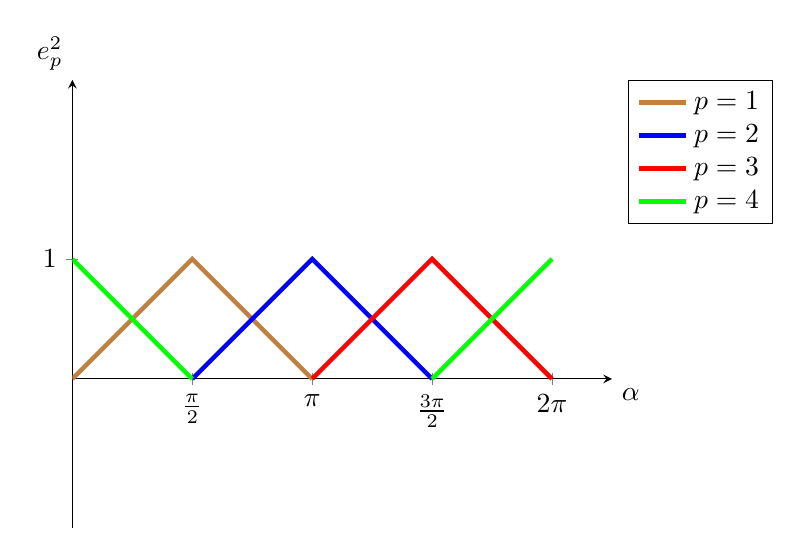
\begin{tikzpicture}
  \begin{axis}[xmax=4.5,
               xmin=0,
               ymin=0,
               ymax=1.25,
               xlabel={$\alpha$},
               ylabel={$e_p^2$},
               xtick={1, 2, 3, 4},
               xticklabels={$\frac{\pi}{2}$, $\pi$, $\frac{3\pi}{2}$, $2\pi$},
               ytick={1},
               axis equal,
               axis x line=center,
               axis y line=center,
               xlabel style={below right},
               ylabel style={above left},
               legend pos=outer north east]
    \addplot [ultra thick, brown] coordinates {(0,0)(1,1)(2,0)};
    \addlegendentry{$p = 1$}
    \addplot [ultra thick, blue] coordinates {(1,0)(2,1)(3,0)};
    \addlegendentry{$p = 2$}
    \addplot [ultra thick, red] coordinates {(2,0)(3,1)(4,0)};
    \addlegendentry{$p = 3$}
    \addplot [ultra thick, green] coordinates {(3,0)(4,1)};
    \addlegendentry{$p = 4$}
    \addplot [ultra thick, green] coordinates {(0,1)(1,0)};
  \end{axis}
\end{tikzpicture}
\end{center}


\subsubsection{Effiziente Berechnung für $K=2$}

Wir können für $K=2$ die Basis-Berechnung durch
\begin{equation}
  e_p^2\left(\alpha\right) = \begin{cases}
    \min\left(\frac{P}{2\pi} \alpha - p + 1, 0\right), & \text{wenn }\alpha \leq t\left(p\right)\text{,}\\
    \min\left(-\frac{P}{2\pi} \alpha + p + 1, 0\right), & \text{sonst}
  \end{cases}
\end{equation}
vereinfachen.

\begin{proof}
  Aufsteigende Gerade der Dreiecksfunktion für $p$, $1 \leq p \leq P$, ist definiert durch
  \begin{equation}
    \frac{\alpha - t\left(p-1\right)}{t\left(p\right) - t\left(p-1\right)} = \frac{P\left(\alpha - t\left(p-1\right)\right)}{2\pi} = \frac{P\alpha - 2\pi\left(p-1\right)}{2\pi} = \frac{P}{2\pi}\alpha - p + 1.
  \end{equation}
  $\min \left(\frac{P}{2\pi} \alpha - p + 1, 0\right)$ beschreibt damit die linke Seite des Dreiecks.
  Analog für absteigende Gerade.
\end{proof}

Die Fallunterscheidung ist unnötig, wir können uns einfach immer für das Minimum der beiden entscheiden.
Die Grafik zeigt dies ziemlich eindeutig.
Das ergibt letztendlich
\begin{equation}
  e_p^2\left(\alpha\right) = \min \left( \min\left(\frac{P}{2\pi} \alpha - p + 1, 0\right), \min\left(-\frac{P}{2\pi} \alpha + p + 1, 0\right) \right)\text{.}
\end{equation}

\begin{figure}
  \centering
  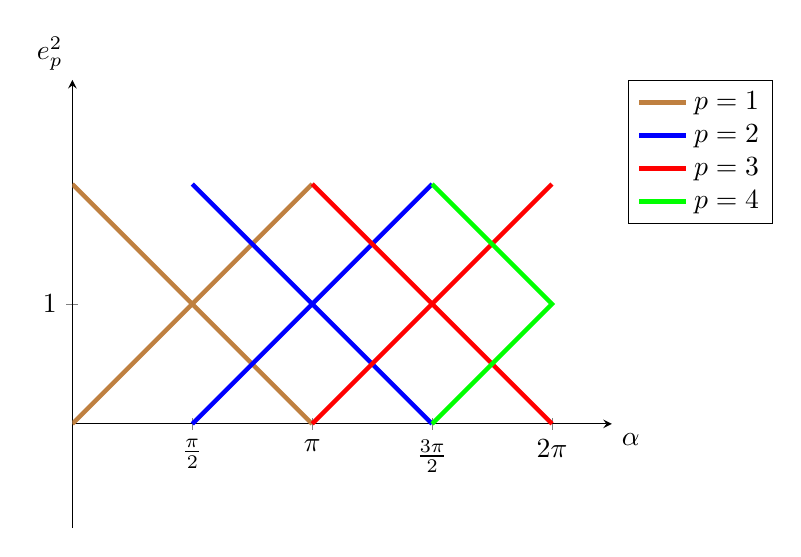
\begin{tikzpicture}
    \begin{axis}[xmax=4.5,
                 xmin=0,
                 ymin=0,
                 ymax=2,
                 xlabel={$\alpha$},
                 ylabel={$e_p^2$},
                 xtick={1, 2, 3, 4},
                 xticklabels={$\frac{\pi}{2}$, $\pi$, $\frac{3\pi}{2}$, $2\pi$},
                 ytick={1},
                 axis equal,
                 axis x line=center,
                 axis y line=center,
                 xlabel style={below right},
                 ylabel style={above left},
                 legend pos=outer north east]
      \addplot [ultra thick, brown] coordinates {(0,0)(2,2)(1,1)(0,2)(2,0)};
      \addlegendentry{$p = 1$}
      \addplot [ultra thick, blue] coordinates {(1,0)(3,2)(2,1)(1,2)(3,0)};
      \addlegendentry{$p = 2$}
      \addplot [ultra thick, red] coordinates {(2,0)(4,2)(3,1)(2,2)(4,0)};
      \addlegendentry{$p = 3$}
      \addplot [ultra thick, green] coordinates {(3,0)(4,1)(3,2)};
      \addlegendentry{$p = 4$}
    \end{axis}
  \end{tikzpicture}
\end{figure}


Wir haben bisher noch nicht den \emph{Kreis} geschlossen mit unserer Formel.

Das können wir aber leicht tun, indem wir unsere absteigenden Geraden um $2\pi$ nach links verschieben und daraus wiederum das Minimum von $0$ ziehen.
Dann sind diese Geraden außer für $p = P$ im Gültigkeitsbereich der Funktion allesamt $0$.
Wir können demnach aus unserer bisherigen Formel und der verschobenen Gerade das Maximum ziehen.
Wir erhalten
\begin{equation}
\begin{split}
  e_p^2\left(\alpha\right) = \max \biggr( & \min \left( \min\left(\frac{P}{2\pi} \alpha - p + 1, 0\right), \min\left(-\frac{P}{2\pi} \alpha + p + 1, 0\right) \right),\\
  & \min \left(-\frac{P}{2\pi} \left( \alpha + 2\pi \right) + p + 1, 0\right) \biggr)\text{.}
\end{split}
\end{equation}

\subsection{Tensorimplementierung}

\begin{equation}
\begin{split}
  \gls{Fout} = & \ {\left(\gls{Adistnorm}\right)}_{ii} \cdot \gls{F} \cdot \ma{W}_{P+1}\\
  & + \sum_{p=1}^P \gls{Adistnorm} \gls{hadamard} e^K_p\left(\gls{Arad}\right) \cdot \gls{F} \cdot \ma{W}_{p}
\end{split}
\end{equation}

\gls{Adistnorm} enthält einmal nur die Diagonale und einmal alles ohne Diagonale.

\newpage


Sei \gls{G} ein Graph im zweidimensionalen euklidschen Raum, eindeutig definiert über dessen Adjazenzmatrizen $\gls{Adist} \in {\left[0, 1\right)}^{N \times N}$ und $\gls{Arad} \in {\left[0, 2\pi\right]}^{N \times N}$.
Dann lässt sich \gls{G} in $P \in \gls{N}$ Bereiche ${\left\{\gls{A}_p\right\}}_{p=1}^P$ \emph{partitionieren}, sodass
\begin{equation*}
  {\left(\gls{A}_p\right)}_{ij} \coloneqq \begin{cases}
    {\left(\gls{Adist}\right)}_{ij}, & \text{wenn } {\left(\gls{Arad}\right)}_{ij} \in \left(\frac{2\pi}{P}\left(p-1\right), \frac{2\pi}{P}p\right]\\
    0, & \text{sonst.}
  \end{cases}
\end{equation*}
Damit beschreiben die Matrizen ${\left\{\gls{A}_p\right\}}_{p=1}^P$ disjunkte Partitionen der Kanten des Graphen \gls{G} abhängig von ihren Ausrichtungen im Raum mit $\gls{Adist} = \sum_{p=1}^P \gls{A}_p$.
$\gls{A}_p$ ist insbesondere nicht zwingend symmetrisch, da ${\left(\gls{Arad}\right)}_{ij} \neq {\left(\gls{Arad}\right)}_{ji}$ für alle $\gls{v}_i, \gls{v}_j \in \gls{V}$ mit $\gls{v}_j \in \gls{Neighbor}\left(\gls{v}_i\right)$.
Abbildung~\ref{fig:partitionierung} veranschaulicht den Prozess der Partitionierung.
Mit $P = 8$ erhalten die jeweiligen Bereiche einen gleichmäßigen Innenwinkel der Größe $\pi/4$.

Es lässt sich analog zu Kapitel~\ref{graph_convolutional_networks} ein Faltungsoperator definieren, bei dem nun aber jeder Partition ein eigener frei trainierbarer Parameter zugeordnet wird.
Der Parameter einer Partition hat damit folglich eine eindeutige Örtlichkeitszuweisung über das Intervall \bzw{} den Bereich der Richtungen seiner Kanten.
Analog zu~\eqref{eq:gcn_renorm} muss dafür zuerst die (Re-)normalisierung der Form
\begin{equation*}
  \gls{Ddisttilde}^{-\frac{1}{2}}\gls{Adisttilde}\gls{Ddisttilde}^{-\frac{1}{2}} = \gls{Ddisttilde}^{-1} + \sum_{p=1}^P \gls{Ddisttilde}^{-\frac{1}{2}}\gls{A}_p\gls{Ddisttilde}^{-\frac{1}{2}}
\end{equation*}
mit $\gls{Adisttilde} \coloneqq \gls{Adist} + \gls{I}$ und ${\left(\gls{Ddisttilde}\right)}_{ii} \coloneqq \sum_{j=1}^N {\left(\gls{Adisttilde}\right)}_{ij}$ durchgeführt werden.
Dies lässt sich mit Hilfe von $\gls{Adist} = \sum_{p=1}^P \gls{A}_p$ und $\gls{Ddisttilde}^{-1/2}\gls{Ddisttilde}^{-1/2} = \gls{Ddisttilde}^{-1}$ verifizieren.
Im Folgenden sei $\gls{Atilde}_p \coloneqq \gls{Ddisttilde}^{-1/2}\gls{A}_p\gls{Ddisttilde}^{-1/2}$ für $p \in \left\{1, \ldots, P \right\}$ und $\gls{Atilde}_0 \coloneqq \gls{Ddisttilde}^{-1}$.
Dann folgt sofort für den Faltungsoperatur $\ve{f}_{\mathrm{in}} \star \ve{\hat g}$ auf Graphen im zweidimensionalen euklidschen Raum, dass dieser
\begin{equation}
  \ve{f}_{\mathrm{in}} \star \ve{\hat g} \approx \sum_{p=0}^P c_p \gls{Atilde}_p \ve{f}_{\mathrm{in}}
  \label{eq:partitionierung_faltung}
\end{equation}
mit den freien Parametern $c_0, \ldots, c_P \in \gls{R}$ erfüllt.

Es stellt sich heraus, dass die Faltung in~\eqref{eq:partitionierung_faltung} auf den Partitionierungen eines regulären Gittergraphen mit $P=8$ äquivalent zu der klassischen Faltung auf einem regulären Gitter mit Filtergröße $3 \times 3$ ist.
\begin{proof}
Sei \gls{G} ein (unendlicher) regulärer Gittergraph bei einer Konnektivität von $8$ und $\ve{f}_{\mathrm{in}}$ Merkmalsvektor auf dem Graphen mit Koordinatenindexnotation ${\left(\ve{f}_{\mathrm{in}}\right)}_{x,y}$.
  Die klassische Faltung \gls{conv2d} an einem Gitterpunkt $\left(x, y\right)$ ist damit gegeben als
\begin{equation*}
  {\gls{conv2d}\left({\ve{f}_{\mathrm{in}}}\right)}_{x,y} = \sum_{i,j \in \left\{1, 2, 3\right\}} {\left(\ve{f}_{\mathrm{in}}\right)}_{x+i-2, y+j-2} \gls{W}_{i, j},
\end{equation*}
wobei $\gls{W} \in \gls{R}^{3 \times 3}$ Filtermatrix der Größe $3 \times 3$.
Da \gls{Adisttilde} ein reguläres Gitter beschreibt sind die Einträge jeder Matrixreihe äquivalent unter unterschiedlicher Permutation und folglich sind die Einträge auf der Diagonalen von \gls{Ddisttilde} identisch (\oBdA{} entfällt hier die Randknotenbetrachtung).
Aufgrund der Partitionierung von \gls{Adist} in $8$ disjunkte Bereiche ${\left\{\gls{Atilde}_p\right\}}_{p=1}^8$ enthält $\gls{Atilde}_p$ genau einen Eintrag pro Matrixreihe korrespondierend zu einer Kante des regulären Gitters.
Für $p \in \left\{2, 4, 6, 8\right\}$ beschreibt $\gls{Atilde}_p$ die horizontalen und vertikalen Kanten des Graphen mit jeweils gleichen Einträgen $\theta_1 \in \gls{R}$.
Analog verweist $\gls{Atilde}_p$ für $p \in \left\{1, 3, 5, 7\right\}$ auf die diagonalen Kanten des Graphen mit den festen Einträgen $\theta_2 \in \gls{R}$.
Sei weiterhin \oBdA{} $\theta_0 \coloneqq {\left(\gls{Ddisttilde}^{-1}\right)}_{ii}$ für beliebiges $i \in \left\{0, \ldots, N\right\}$.
Mit der Zuordnung
\begin{equation*}
  \gls{W} = \begin{bmatrix}
    c_7\theta_2 & c_8\theta_1 & c_1\theta_2\\
    c_6\theta_1 & c_0\theta_0 & c_2\theta_1\\
    c_5\theta_2 & c_4\theta_1 & c_3\theta_2
  \end{bmatrix}
\end{equation*}
für die Faltung $\ve{f}_{\mathrm{in}} \star \ve{\hat g}$ aus~\eqref{eq:partitionierung_faltung} mit den Parametern $c_0, \ldots, c_8 \in \gls{R}$
folgt damit sofort die Äquivalenz zu $\gls{conv2d}\left(\ve{f}_{\mathrm{in}}\right)$ auf regulären Gittern.
\end{proof}

\paragraph{Implementierung}
\label{partitionierung_implementierung}

\begin{equation}
  \ma{F}_{\mathrm{out}} \coloneqq \sum_{p=0}^P \gls{Atilde}_p\ma{F}_{\mathrm{in}}\gls{W}_p
\end{equation}
wadawd
\\\\
Obwohl
Eine Lösung zu diesem Problem ist die Interpolation der Innenwinkel über die Basisfunktionen einer B-Spline-Kurve.

% \begin{equation}
%   f^{\prime}_{iy} = \sum_{x = 1}^X \tilde a_{ii} \cdot f_{ix} \cdot w_{\left(P +1\right)xy} \sum_{n = 1, n \neq i}^N \tilde a_{in} \cdot f_{nx} \cdot b^K_P\left(\alpha_{in}, x, y\right)
% \end{equation}
% wobei $b_P^K$ eine B-Spline-Kurve.
% \todo{$a_{ii}$ kann raus, da immer $1$}

% Es ist anzumerken, dass im Summanden der betrachtete Knoten übersprungen wird, da für diesen ein Wert in der Winkelmatrix keinen Sinn ergibt.
% Er wird daher in der Faltung jeweils einzeln mit einem Gewicht multipliziert und dazuaddiert.

% \paragraph{B-Spline-Kurven}
% \label{bspline}

% $b_P^K \colon \left(0, 2\pi\right]\to\gls{R}$ ist eine \emph{B-Spline-Kurve} der Ordnung $K \in \gls{N}$ mit $P \in \gls{N}$ Kontrollpunkten auf den Kantenwinkeln $\left(0, 2\pi\right]$ eines Graphknotens $\gls{v}_i$ zu seinen adjazenten Knoten $\gls{v}_j$.
% Es ist wichtig anzumerken, dass Null für Winkel ausgeschlossen werden und stattdessen der Winkel $2\pi$ benutzt wird, so dass wir nicht mit der Bedeutung von $0$ in Adjazenzmatrizen in die Quere kommen.
% \\\\
% \begin{equation}
%   b_P^K\left(\alpha, x, y \right) = \sum_{p=1}^P w_{pxy} \cdot e_p^K\left(\alpha\right)
% \end{equation}
% wobei die Basisfunktion $e_p^K$ rekursiv über $K$ definiert ist mit Initialisierung
% \begin{equation}
%   e_p^1\left(\alpha\right) = \begin{cases}
%     1, & \text{wenn }\alpha \in \left] t\left(p-1\right), t\left(p\right)\right]\text{,}\\
%     0, & \text{sonst}
%   \end{cases}
% \end{equation}
% und Rekursionsschritt
% \begin{equation}
%   e_p^k\left(\alpha\right) = \frac{\alpha - t\left(p - 1\right)}{t\left(p+k-2\right) - t\left(p - 1\right)} e_p^{k-1}\left(\alpha\right) + \frac{t\left(i\left(p + k - 1\right)\right) - \alpha}{t\left(p+k - 1\right) - t\left(p\right)} e_{i\left(p+1\right)}^{k-1}\left(\alpha\right)
% \end{equation}
% wobei $t \colon \gls{N} \to \gls{R}$ mit $t\left(p\right) = 2\pi\frac{p}{P}$ und $i\left(p\right) = \gls{modulo}\left(p-1, P\right) + 1$.
% Es ist anzumerken, dass wir $t$ und $i$ dabei für den Rekursionsschritt über die Grenze $P$ hinaus definieren.
% Das hilft uns, die B-Spline-Kurve \emph{kreisförmig} abzuschließen.

% Je größer $K$ gesetzt wird, umso mehr Anteile anderer benachbarter Stützpunkte fließen in die Berechnung mit ein.
% Die Größe von $K$ wird deshalb auch oft \emph{lokale Kontrollierbarkeit} genannt.

% \paragraph{Faltungsoperator}
% \label{ebener_faltungsoperator}

\begin{figure}[t]
\centering
  \subfigure[$\gls{G}_0$]{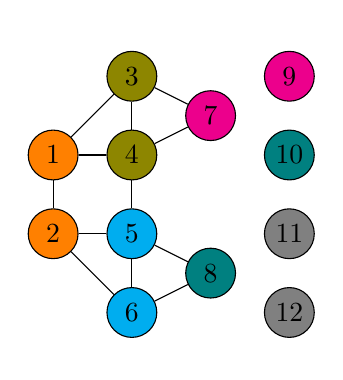
\begin{tikzpicture}
  \fill [white] (-1, -2) rectangle (1, 2) node {};  % Zentriere Graph.
  \tikzstyle{node}=[circle,draw, minimum width=18pt, inner sep=0pt, fill=white]
  \tikzstyle{color1}=[fill=orange]
  \tikzstyle{color2}=[fill=olive]
  \tikzstyle{color3}=[fill=cyan]
  \tikzstyle{color4}=[fill=magenta]
  \tikzstyle{color5}=[fill=teal]
  \tikzstyle{color6}=[fill=gray]

  \node[node, color1] (1)  at (-2, 0.5)  {$1$};
  \node[node, color1] (2)  at (-2, -0.5) {$2$};
  \node[node, color2] (3)  at (-1, 1.5)  {$3$};
  \node[node, color2] (4)  at (-1, 0.5)  {$4$};
  \node[node, color3] (5)  at (-1, -0.5) {$5$};
  \node[node, color3] (6)  at (-1, -1.5) {$6$};
  \node[node, color4] (7)  at (0,  1)    {$7$};
  \node[node, color5] (8)  at (0,  -1)   {$8$};

  \node[node, color4] (9)  at (1, 1.5)   {$9$};
  \node[node, color5] (10) at (1, 0.5)   {$10$};
  \node[node, color6] (11) at (1, -0.5)  {$11$};
  \node[node, color6] (12) at (1, -1.5)  {$12$};

  \path (1) edge (2);
  \path (1) edge (3);
  \path (1) edge (4);
  \path (2) edge (5);
  \path (2) edge (6);
  \path (3) edge (4);
  \path (3) edge (7);
  \path (4) edge (5);
  \path (4) edge (7);
  \path (5) edge (6);
  \path (5) edge (8);
  \path (6) edge (8);
\end{tikzpicture}
}
\hspace{1cm}
  \subfigure[$\gls{G}_1$]{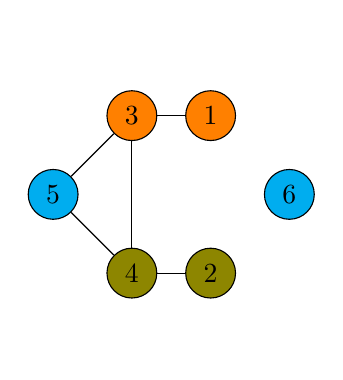
\begin{tikzpicture}
  \fill [white] (-1, -2) rectangle (1, 2) node {};  % Zentriere Graph.
  \tikzstyle{node}=[circle,draw, minimum width=18pt, inner sep=0pt, fill=white]
  \tikzstyle{color1}=[fill=orange]
  \tikzstyle{color2}=[fill=olive]
  \tikzstyle{color3}=[fill=cyan]

  \node[node, color3] (1) at (-1, 0) {$5$};
  \node[node, color1] (2) at (0,  1) {$3$};
  \node[node, color2] (3) at (0, -1) {$4$};
  \node[node, color1] (4) at (1,  1) {$1$};
  \node[node, color2] (5) at (1, -1) {$2$};

  \node[node, color3] (6) at (2, 0)  {$6$};

  \path (1) edge (2);
  \path (1) edge (3);
  \path (2) edge (3);
  \path (2) edge (4);
  \path (3) edge (5);
\end{tikzpicture}
}
\hspace{1cm}
  \subfigure[$\gls{G}_2$]{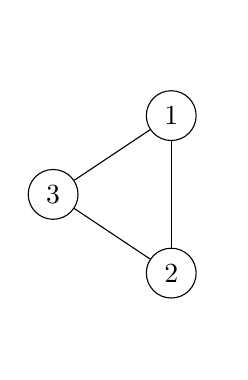
\begin{tikzpicture}
  \fill [white] (-1, -2) rectangle (1, 2) node {};  % Zentriere Graph.
  \tikzstyle{node}=[circle,draw, minimum width=18pt, inner sep=0pt, fill=white]

  \node[node] (1) at (-1,   0) {$3$};
  \node[node] (2) at (0.5,  1) {$1$};
  \node[node] (3) at (0.5, -1) {$2$};

  \path (1) edge (2);
  \path (1) edge (3);
  \path (2) edge (3);
\end{tikzpicture}
}
\hspace{1cm}
  \subfigure[Anorderung der Knoten zu einem binären Baum]{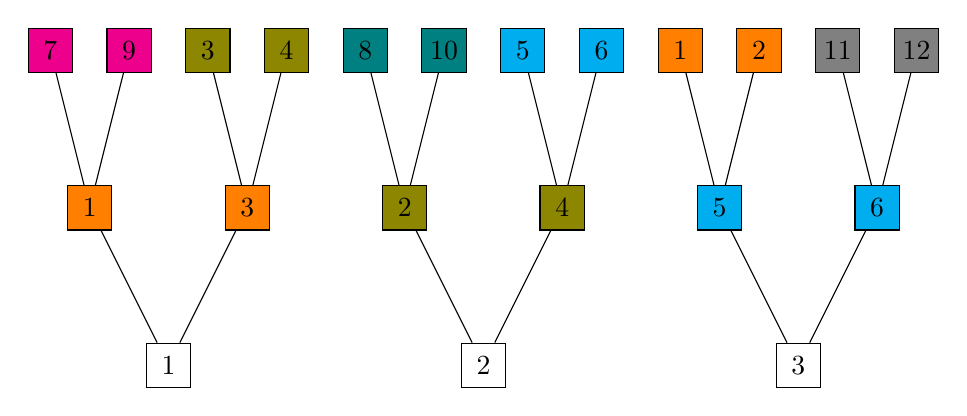
\begin{tikzpicture}
  \tikzstyle{node}=[rectangle,draw, minimum width=16pt, minimum height=16pt, inner sep=0pt, fill=white]
  \tikzstyle{color1}=[fill=orange]
  \tikzstyle{color2}=[fill=olive]
  \tikzstyle{color3}=[fill=cyan]
  \tikzstyle{color4}=[fill=magenta]
  \tikzstyle{color5}=[fill=teal]
  \tikzstyle{color6}=[fill=gray]

  \node[node, color4] (01)  at (-5.5, 2) {$7$};
  \node[node, color4] (02)  at (-4.5, 2) {$9$};
  \node[node, color2] (03)  at (-3.5, 2) {$3$};
  \node[node, color2] (04)  at (-2.5, 2) {$4$};
  \node[node, color5] (05)  at (-1.5, 2) {$8$};
  \node[node, color5] (06)  at (-0.5, 2) {$10$};
  \node[node, color3] (07)  at (0.5,  2) {$5$};
  \node[node, color3] (08)  at (1.5,  2) {$6$};
  \node[node, color1] (09)  at (2.5,  2) {$1$};
  \node[node, color1] (010) at (3.5,  2) {$2$};
  \node[node, color6] (011) at (4.5,  2) {$11$};
  \node[node, color6] (012) at (5.5,  2) {$12$};

  \node[node, color1] (11) at (-5, 0) {$1$};
  \node[node, color1] (12) at (-3, 0) {$3$};
  \node[node, color2] (13) at (-1, 0) {$2$};
  \node[node, color2] (14) at (1,  0) {$4$};
  \node[node, color3] (15) at (3,  0) {$5$};
  \node[node, color3] (16) at (5,  0) {$6$};

  \node[node] (21) at (-4, -2)  {$1$};
  \node[node] (22) at (0,  -2)  {$2$};
  \node[node] (23) at (4,  -2)  {$3$};

  \path (21) edge (11);
  \path (21) edge (12);
  \path (22) edge (13);
  \path (22) edge (14);
  \path (23) edge (15);
  \path (23) edge (16);
  \path (11) edge (01);
  \path (11) edge (02);
  \path (12) edge (03);
  \path (12) edge (04);
  \path (13) edge (05);
  \path (13) edge (06);
  \path (14) edge (07);
  \path (14) edge (08);
  \path (15) edge (09);
  \path (15) edge (010);
  \path (16) edge (011);
  \path (16) edge (012);
\end{tikzpicture}
}
\caption[Pooling auf Graphen]{Illustration einer Pooling-Operationen der Größe $4$ (\bzw{} zweier Pooling-Operationen der Größe $2$) auf einem Graphen \gls{G} der Größe $\left|\gls{V}\right| = 8$.
Das Clustering von \gls{G} liefert uns im ersten Schritt $N_1 =\left|\gls{V}_1\right| = 5$ Knoten und im darauf folgenden $N_2 = \left|\gls{V}_2\right| = 3$ Knoten.
Die Größen der Graphen werden daraufhin zu $N_2 = 3$, $N_1 = 6$ und $N_0 = 12$ angepasst, so dass jeder Knoten auf genau $2$ Vorgängerknoten verweist, indem \enquote{Fake}-Knoten zu $\gls{G}_1$ (1 Knoten) und $\gls{G}_0$ (4 Knoten) hinzugefügt werden.
Mit der Anordnung der Knoten zu einem binären Baum (d) kann die Pooling-Operation $\max\left(\cdot\right)$ eines Signals $\ve{f} \in \gls{R}^{12}$ auf $\gls{G}_0$ dann effizient als $\ve{f}_{\mathrm{pool}} \coloneqq {\left[ \max\left(\ve{f}_1, \ve{f}_2, \ve{f}_3, \ve{f}_4 \right), \max\left(\ve{f}_5, \ve{f}_6, \ve{f}_7, \ve{f}_8 \right), \max\left(\ve{f}_9, \ve{f}_{10}, \ve{f}_{11}, \ve{f}_{12} \right) \right]}^{\top} \in \gls{R}^3$ implementiert werden, wobei die Werte der \enquote{Fake}-Knoten $\ve{f}_2, \ve{f}_6, \ve{f}_{11}, \ve{f}_{12}$ auf den neutralen Wert $0$ der \gls{relu}-Aktivierungsfunktion gesetzt werden.}
\label{fig:pooling}
\end{figure}

\section{Netzarchitektur}
\label{raeumliche_netzarchitektur}

% Hier den Cube vorstellen
% 1D Convolutions etc

\begin{figure}[t]
\centering
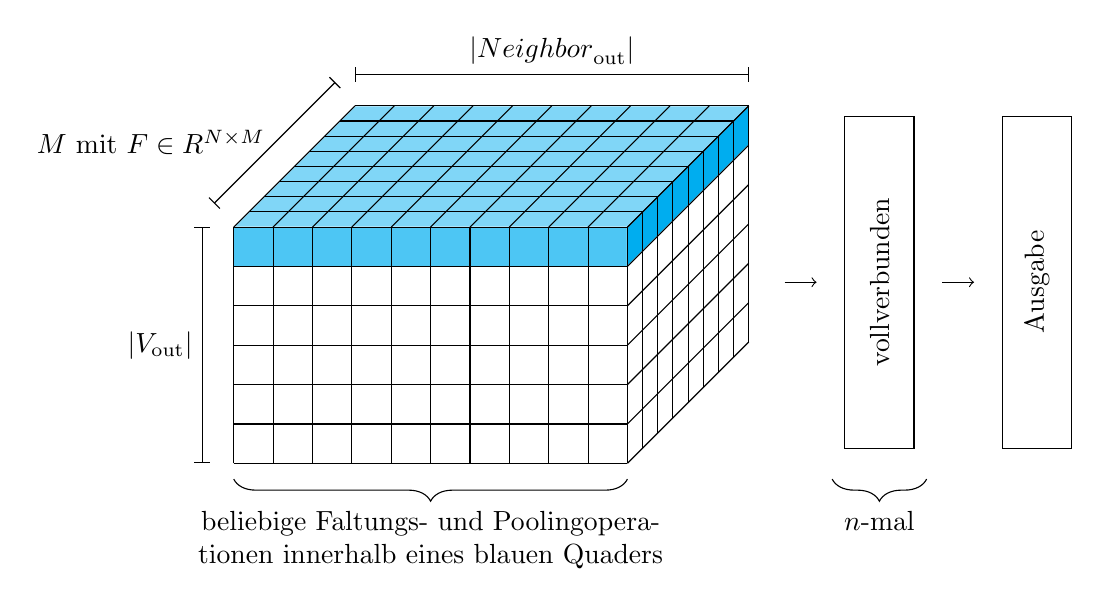
\begin{tikzpicture}
  \draw[white,fill=cyan!70] (0, 3, 4) -- (5, 3, 4) -- (5, 2.5, 4) -- (0, 2.5, 4) -- cycle;
  \draw[white,fill=cyan!50] (0, 3, 4) -- (5, 3, 4) -- (5, 3,   0) -- (0, 3,   0) -- cycle;
  \draw[white,fill=cyan]    (5, 3, 4) -- (5, 3, 0) -- (5, 2.5, 0) -- (5, 2.5, 4) -- cycle;
  \tikzstyle{path}=[->, shorten >= 10pt, shorten <= 10pt]
  \tikzstyle{node}=[rectangle,draw, minimum width=120pt, minimum height=25pt, inner sep=0pt, fill=white, rotate=90]
  \tikzstyle{noborder}=[draw=none,fill=none]

  \foreach \x in {0,0.5,1,1.5,2,2.5,3} {%
    \draw (0,  \x, 4)  -- (5,  \x, 4);
    \draw (5,  \x, 4)  -- (5,  \x, 0);
  }
  \foreach \x in {0,0.5,1,1.5,2,2.5,3,3.5,4,4.5,5} {%
    \draw (\x, 0,  4)  -- (\x, 3,  4);
    \draw (\x, 3,  4)  -- (\x, 3,  0);
  }
  \foreach \x in {0,0.5,1,1.5,2,2.5,3,3.5,4} {%
    \draw (5,  0,  \x) -- (5,  3, \x);
    \draw (0,  3,  \x) -- (5,  3, \x);
  }

  \draw[|-|] (-0.4, 0,    4)    -- node[left]  {$\left|\gls{V}_{\mathrm{out}}\right|$}        (-0.4, 3,    4);
  \draw[|-|] (0,    3.55, 4.65) -- node[left]  {$M$ mit $\ma{F} \in \gls{R}^{N \times M}$}    (0,    3.55, 0.65);
  \draw[|-|] (0,    3.4,  0)    -- node[above] {$\left|\gls{Neighbor}_{\mathrm{out}}\right|$} (5,    3.4,  0);

  \node[node, noborder] (0) at (6.2,  2.3, 4) {};
  \node[node]           (1) at (8.2,  2.3, 4) {vollverbunden};
  \node[node]           (2) at (10.2, 2.3, 4) {Ausgabe};

  \path[path] (0) edge (1);
  \path[path] (1) edge (2);

  \draw [decoration={brace,mirror,amplitude=8pt},decorate,-] (0,-0.2,4) -- node[below=8pt,text width=8cm, align=center] {beliebige Faltungs- und Poolingoperationen innerhalb eines blauen Quaders} (5,-0.2,4);
  \draw [decoration={brace,mirror,amplitude=8pt},decorate,-] (7.6,-0.2,4) -- node[below=8pt] {$n$-mal} (8.8,-0.2,4);

\end{tikzpicture}
\caption[Räumliche Netzarchitektur auf Graphen]{Typische räumliche Netzarchitektur auf Graphen.
Der \emph{Quader}, der durch die Anordnung der Knoten entsprechend ihrer Nachbarschaften entsteht, kann entlang der Nachbarschaften und ihrer Merkmale beliebig oft gefaltet und gepoolt werden.
Eine Faltung entlang der Knotenauswahl besitzt allerdings keine Bedeutung und ist deshalb zu vermeiden.
Im Anschluss können vollverbundene Schichten hin zur Ausgabe an den abgeflachten Quader gestapelt werden.}
\label{fig:netzarchitektur_raeumlich}
\end{figure}


Eigentliche Graphstruktur geht verloren (\zB{} Distanzen der Knoten zueinander) (in gewisser weise stecken diese aber in den Formfeatures).

Die Anordnung der Knoten zu einem Quaderform besitzt damit die Einschränkung, dass das Netz lediglich eine Faltungsschicht enthalten kann.
Die Methode der spektralen Faltung auf Graphen umgeht diese Einschränkung.

Würfel ist speicherineffizient

